\documentclass{article}

% Formatting
\usepackage[utf8]{inputenc}
\usepackage[margin=1in]{geometry}
\usepackage[titletoc,title]{appendix}

% Math
\usepackage{amsmath,amsfonts,amssymb,mathtools}

% Algorithms
\usepackage[ruled,vlined]{algorithm2e}
\usepackage{algorithmic}
\usepackage{listings}

% Code syntax highlighting
\usepackage{minted}
\usemintedstyle{borland}

% Tree & Forest
\usepackage[edges]{forest}

\title{Homework 4}
\author{David Trinh}
\date{October 14, 2024}

\begin{document}

\maketitle

\begin{itemize}

    \item\textbf{ Question 1}

    \begin{lstlisting}
class Node:
    private value
    private next

    constructor(value):
        this.value = value
        this.next = null

class LinkedList:
    private head
    private tail
    private length

    constructor():
        this.head = null
        this.tail = null
        this.size = 0

    public method length():
        return this.size
    
    public method isEmpty():
        if this.size == 0:
            return True
        else:
            return False

    // Insert at the tail of the list
    public method insert(value):
        node = new Node(value)
        if this.head is null do
            this.head = node
            this.tail = node
        else do
            this.tail.next = node
            this.tail = this.tail.next

        this.size = this.size + 1
    
    // Returns the first occurrence of the value
    public method find(value):
        if this.isEmpty():
            return null

        current = this.head
        while current is not null do
            if current.value == value do
                return current

            current = current.next
        
        return null

    // Only deletes the first occurrence of the value
    public method delete(value):
        if this.isEmpty() do
            return null
        
        current = this.head
        if this.length == 1 and current.value == value do
            this.head = null
            this.tail = null
            this.size = 0
            return current

        previous = null
        while current is not null do
            if current.value == value do
                previous.next = current.next
                this.length = this.length - 1
                return current

            previous = current
            current = current.next
        
        return null


    \end{lstlisting}

    \item\textbf{ Question 2}

    \begin{itemize}
        \item[] Description of accepted strings:
            \begin{itemize}
                \item Assume that any combination includes empty string
                \item Starts with any combination of b's and c's
                \item Has the definite string abc in the middle
                \item Ends with any combination of a's and b's
            \end{itemize}

        \item[] accept:     bccabcbaab, abc

        \item[] rejected:   cab, bcabcb

        \item[] $[bc]*abc[ab]*$

        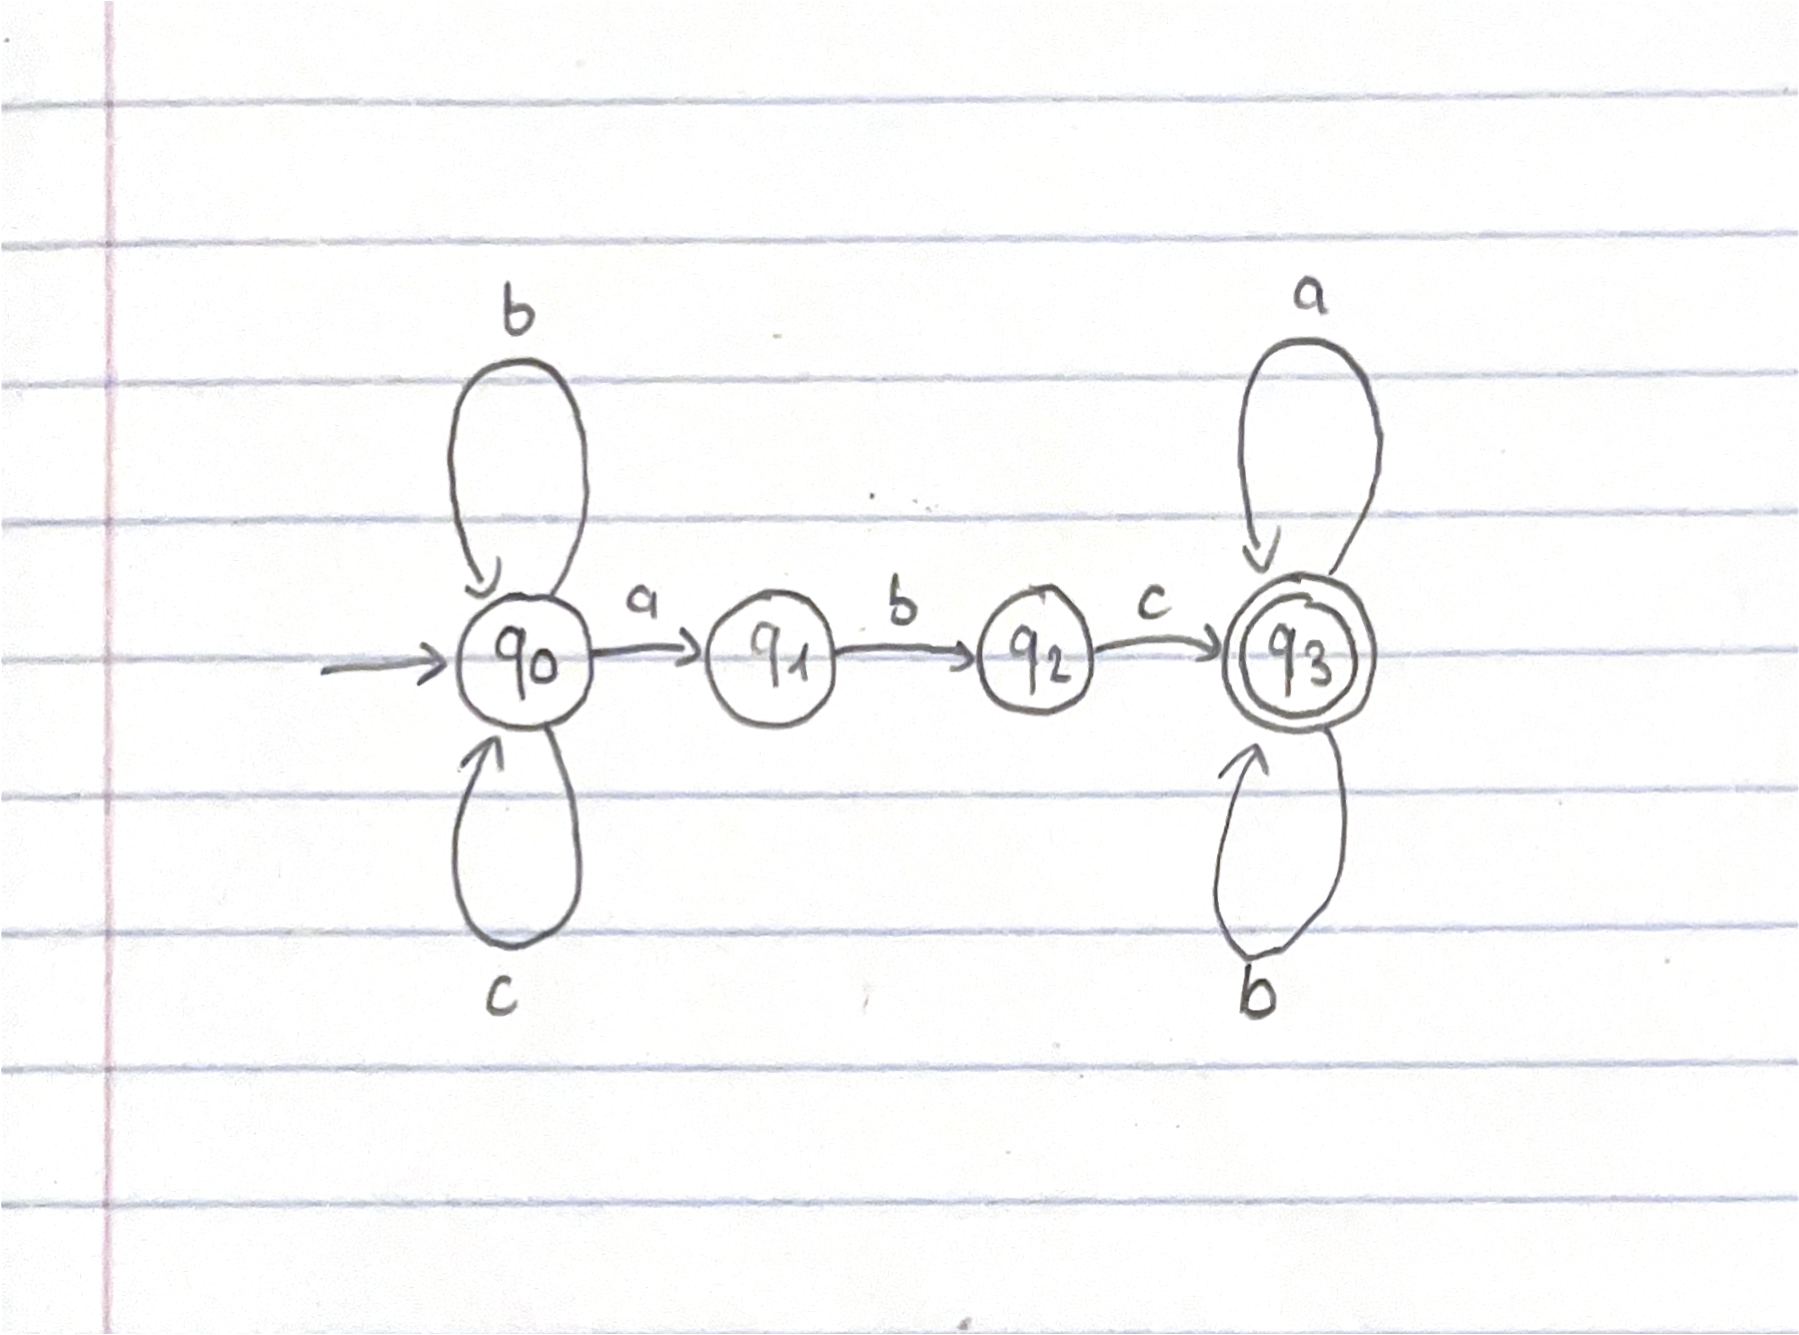
\includegraphics[scale=0.2]{Quiz2_Q2.png}

    \end{itemize}
    


    \item\textbf{ Question 3}

    The output is capped at 13 characters, including:

    \begin{itemize}
        \item Capital letters A to Z: 26
        \item Non-capital letters a to z: 26
        \item Digits 0 to 9: 10
    \end{itemize}

    An output of 13 characters, each with 62 possible alphanumeric character would yield $62^{13} = 2 \times 10^{23}$ unique shortened URLs. This is more than plenty. Assuming that the number of URLs in the world is less than $2 \times 10^{23}$ (most likely), we can implement a hashing algorithm to generate unique shortened URLs.

    The only rule our hashing algorithm requires is that all shortened URL are unique, such that each will link to only one real URL. In that spirit, having a counter from "0000000000000" to "ZZZZZZZZZZZZZ" will work fine. This is because there isn't much of a security concern. However, it doesn't hurt to implement a hashing algorithm like SHA256 and take the first $6 * 13 = 78$ bits to generate a 13 character string, 6 bits for each alphanumeric character.
    
    Then, we can create a HashTable where the keys are the shortened string and the values are the real URL. Whenever a user search for tinyurl.com/xxxxxxxxxxxxx, the server will look at the value (real URL) assigned to the key xxxxxxxxxxxxx in the database HashTable and redirect them there.



\end{itemize}

\end{document}